\documentclass[conference]{IEEEtran}

% NILES2026 submission — anonymous, 4-page limit, no page numbers/headers/footers.
% Condensed from paper.tex; that file remains the full-length version.

\usepackage[utf8]{inputenc}
\usepackage[english]{babel}
\usepackage{lmodern}

\usepackage{amsmath, amssymb}
\usepackage{graphicx}
\usepackage{subcaption}
\usepackage{booktabs}

\usepackage{listings}
\usepackage{xcolor}
\lstset{
  basicstyle=\ttfamily\small,
  keywordstyle=\color{blue},
  commentstyle=\color{gray},
  frame=single,
  breaklines=true,
}

\usepackage{algorithm}
\usepackage{algpseudocode}

\usepackage{tikz}
\usetikzlibrary{arrows.meta, shapes.geometric, positioning, fit, backgrounds}

\usepackage[hidelinks]{hyperref}
\usepackage{cleveref}
\crefname{lstlisting}{Listing}{Listings}

% ── Metadata ──────────────────────────────────────────────────────────────────
\title{LLM-Driven Algorithmic Trading: A Reinforcement Learning Fine-Tuning Framework}

% Anonymized for double-blind review per NILES2026 requirements.
\author{
  \IEEEauthorblockN{Anonymous Authors}
  \IEEEauthorblockA{Details omitted for double-blind review}
}

\begin{document}

\maketitle

\begin{abstract}
This paper presents a reinforcement learning fine-tuning framework for LLM-driven algorithmic
trading, training open-source large language models to generate executable Python trading
strategies via Group Relative Policy Optimisation (GRPO).
We fine-tune Qwen2.5-7B, Qwen2.5-32B, and Llama-3.1-8B and evaluate their strategy generation
performance and trading outcomes across 38 equities.
Our results demonstrate that fine-tuning significantly enhances model performance,
with an average increase of 82\% in strategy generation accuracy and a 250\% improvement in trading returns compared to base models.
These findings underscore the potential of reinforcement learning fine-tuning in aligning LLM outputs with complex financial objectives,
paving the way for more effective and adaptive algorithmic trading systems.
\end{abstract}

\begin{IEEEkeywords}
large language models, reinforcement learning, algorithmic trading, GRPO, fine-tuning, strategy generation
\end{IEEEkeywords}

% ── Section 1 – Introduction ──────────────────────────────────────────────────
\section{Introduction}
\label{ch:intro}

Financial markets are complex, nonlinear, and dynamic systems whose stochastic price
movements, high volatility, and non-stationarity make modelling and decision-making
particularly challenging. Traditional rule-based and static statistical models often
struggle with changing market conditions, motivating intelligent systems that learn and
adapt under uncertainty. Machine-learning approaches to algorithmic trading broadly fall
into \emph{prediction-based} and \emph{reinforcement learning-based} methods; this paper
focuses on the latter.

Formally, given a financial instrument $s$ and a historical price series
$\mathcal{D}_s = \{p_1, p_2, \ldots, p_T\}$, the objective is to learn a policy $\pi_\theta$ that,
conditioned on a prompt $p(s)$, generates an executable trading strategy
$o \sim \pi_\theta(\cdot \mid p(s))$ that maximises the expected annualised return when evaluated
on an out-of-sample period:
\begin{equation}
  \max_\theta \; \mathbb{E}_{s \sim \mathcal{S}}\bigl[R(\pi_\theta, s)\bigr]
\end{equation}
where $R(\pi_\theta, s)$ denotes the annualised return of the generated strategy on symbol $s$, and
$\mathcal{S}$ is the set of target financial instruments.

This paper investigates the following research questions:
\begin{enumerate}
  \item[\textbf{RQ1}] Does Group Relative Policy Optimisation (GRPO) fine-tuning significantly improve a model's ability to generate
    syntactically valid and executable trading strategies compared to its base counterpart?
  \item[\textbf{RQ2}] Does fine-tuning improve the financial performance of generated strategies
    in terms of annualised return and Sharpe ratio?
  \item[\textbf{RQ3}] How does the effectiveness of GRPO fine-tuning vary across model families
    and parameter scales?
\end{enumerate}

Despite the rapid growth of research applying large language models (LLMs) to financial
trading, existing studies primarily rely on standard pretrained or fine-tuned LLMs for
prediction, sentiment analysis, or agent-based decision making. As far as our review
indicates, little to no work either incorporates LLMs to generate executable trading
strategies or employs GRPO or Reinforcement Learning with Verifiable Rewards (RLVR) to
fine-tune them for this purpose.
Our contributions are: (i) a novel framework for trading strategy generation using large
language models; (ii) a backtesting environment for evaluating generated strategies on
historical market data; (iii) the application of GRPO to specialise a language model for
strategy generation; and (iv) empirical comparisons across multiple models and benchmarks
demonstrating the effectiveness of our approach.

% ── Section 2 – Related Work ──────────────────────────────────────────────────
\section{Related Work}
\label{ch:related}

\subsection{Machine Learning for Trading}
Prediction-based methods forecast asset prices from historical data, technical
indicators, and sentiment signals, with LSTM~\cite{hochreiter1997lstm} variants and
hybrid attention architectures dominating the literature~\cite{huang2024novel}. However,
higher prediction accuracy does not guarantee higher returns~\cite{huang2024novel}, and
practitioners must still construct strategies around forecasts. Reinforcement
learning~\cite{sutton2018rl} instead optimises trading decisions directly: value-based
methods are the most widely adopted for single-asset trading~\cite{huang2024novel}, while
policy-gradient and actor-critic algorithms directly optimise the policy.

\subsection{LLMs in Financial Trading}
LLM applications in equity markets have grown rapidly since
ChatGPT~\cite{achiam2023gpt4}, spanning price prediction, sentiment analysis, automated
trading, portfolio and risk management, and benchmarking~\cite{jadhav2025llmequity}. Trading-focused implementations are broadly
categorised~\cite{ding2024survey} into \emph{LLMs as traders}, which directly generate
buy/hold/sell decisions, and \emph{LLMs as alpha miners}, which generate quantitative
predictive signals. Trader-style agents include memory-and-reflection architectures such
as FinMem~\cite{yu2023finmem} and the multimodal FinAgent~\cite{zhang2024finagent}, and
reinforcement-learning-driven systems~\cite{koa2024explainable,ding2023}. Alpha-mining
frameworks \cite{wang2024quantagent,wang2023alphagpt} iteratively generate and backtest
signal scripts, progressively refining an agent's knowledge base. Our approach differs
from both: we prompt the model to generate complete executable trading strategies rather
than decisions or isolated signals.

\subsection{Reinforcement Fine-Tuning}
Reinforcement fine-tuning (RFT) adapts a pretrained model using a scalar feedback signal:
an algorithmic grader scores model outputs, and weights are updated to increase the
likelihood of high-scoring responses~\cite{openai2024rft}. Parameter-efficient methods
such as LoRA~\cite{hu2021lora} make this feasible on limited hardware, and
FinGPT~\cite{liu2023fingpt} couples them with market feedback for financial applications.
Closest to our work,
RLMF~\cite{saqur2024} uses market price signals as rewards to update a Llama-2 7B model;
SCRL~\cite{ding2023} fine-tunes a Llama 7B via PPO to align news embeddings with stock
features; and SEP~\cite{koa2024explainable} applies PPO to fine-tune an LLM to generate
self-reflective explanations of past stock movements. None of these generate executable
strategies or employ GRPO.

% ── Section 3 – Methodology ───────────────────────────────────────────────────
\section{Methodology}
\label{ch:method}

\subsection{Algorithm}
\label{sec:algorithm}

In our setting the \emph{environment} is the financial market,
the \emph{action} is the trading strategy generated by the model in response to a prompt,
and the \emph{reward} is the return generated by the strategy when back-tested on
historical data. Reinforcement learning from human feedback
(RLHF)~\cite{christiano2017rlhf}, typically implemented with Proximal Policy Optimisation
(PPO)~\cite{schulman2017ppo}, optimises a policy against a learned reward model but
requires training and maintaining both a reward model and a value model alongside the
policy. Group Relative Policy Optimisation (GRPO)~\cite{shao2024deepseekmath} makes two
key simplifications: the value model is removed entirely, and the learned reward model is
replaced by an algorithmically verifiable reward function---a paradigm known as
Reinforcement Learning with Verifiable Rewards (RLVR). In place of the value model, GRPO estimates the advantage by sampling the
policy $G$ times for the same prompt and computing the Z-score of the resulting rewards:
\begin{equation}
  A_i = \frac{r_i - \operatorname{mean}(r_1, r_2, \ldots, r_G)}
             {\operatorname{std}(r_1, r_2, \ldots, r_G)},
  \label{eq:grpo-advantage}
\end{equation}
where $r_i$ is the reward assigned to the $i$-th sample. The GRPO objective is
\begin{multline}
  \mathcal{L}(\theta) = \tfrac{1}{G}\sum_{i=1}^{G}
    \min\!\bigl(\rho_i\hat{A}_i,\,
      \mathrm{clip}(\rho_i,1{-}\varepsilon,1{+}\varepsilon)\hat{A}_i\bigr) \\
    - \beta D_{\mathrm{KL}}(\pi_\theta\|\pi_{\mathrm{ref}}),
  \label{eq:grpo-obj}
\end{multline}
where $\rho_i = \pi_\theta(o_i \mid p)/\pi_{\theta_\text{old}}(o_i \mid p)$, $\varepsilon$
is a clipping hyperparameter that prevents excessively large policy updates, and
$\beta > 0$ weights a KL-divergence penalty constraining deviation from the reference
policy. RLVR suits tasks with easily verifiable solutions such as mathematics and code
generation; financial strategy evaluation, while more nuanced, is likewise
\emph{verifiable}---a strategy either produces positive back-tested returns or it does
not---making GRPO appropriate for our setting.

\subsection{System Overview}
\label{sec:system}

Our implementation uses the \texttt{Unsloth} library \cite{unsloth2024} to load and
fine-tune the language model. Each training step proceeds as follows: a symbol
$s \sim \mathcal{S}$ is sampled and a prompt $p(s)$ constructed; the LLM generates $G$
candidate trading strategies; the backtesting module evaluates each candidate and maps the
result to a scalar reward (\cref{tab:reward}); group-relative advantages are computed via
\cref{eq:grpo-advantage}; and the policy is updated by ascending the GRPO objective in
\cref{eq:grpo-obj}.

\paragraph{Strategy generation.}
The model is prompted to generate a single-asset trading strategy for a given symbol and
date range. The prompt, iteratively refined with the assistance of a frontier language
model, imposes strict output constraints: the response must consist solely of a Python
subclass of the Backtrader \texttt{bt.Strategy} class named \texttt{Strategy} (simplifying
extraction), with all indicators created in \texttt{\_\_init\_\_}, trading logic in
\texttt{next()}, and orders restricted to \texttt{buy}, \texttt{sell}, \texttt{close}, and
\texttt{order\_target\_percent}. Imports and external references (data files, APIs, or
indicators outside Backtrader) are prohibited to prevent look-ahead bias and reduce
execution errors. An example output
from the fine-tuned Qwen2.5-32B model for TSLA is shown in \cref{lst:tsla-strategy}.

\begin{figure}[t]
\begin{lstlisting}[language=Python,
                   caption={Example strategy generated by Qwen2.5-32B (fine-tuned) for TSLA.},
                   label={lst:tsla-strategy},
                   basicstyle=\ttfamily\footnotesize]
class Strategy(bt.Strategy):
    def __init__(self):
        self.sma20 = bt.indicators.SimpleMovingAverage(
            self.data.close, period=20)
        self.sma50 = bt.indicators.SimpleMovingAverage(
            self.data.close, period=50)

    def next(self):
        if self.sma20 > self.sma50:
            self.order_target_percent(target=1.0)
        elif self.sma20 < self.sma50:
            self.order_target_percent(target=0.0)
\end{lstlisting}
\end{figure}

\paragraph{Back-testing.}
Once the model produces an output, the strategy class is extracted via regex and passed
to our back-testing setup built on \texttt{Backtrader} \cite{backtrader2024}. Look-ahead
bias is prohibited by the prompt constraints and enforced by the Backtrader execution
environment.

\paragraph{Reward function.}
The back-test result is mapped to a scalar reward according to the hierarchy in
\cref{tab:reward}. Outcomes 1--3 are penalised to discourage invalid outputs: the model
must first learn to produce correct Backtrader strategies. Negative returns receive zero
rather than a negative reward, as they remain preferable to invalid or signal-free
outputs, while positive returns earn the annualised return $R$, rewarding more profitable
strategies proportionally.

\begin{table}[t]
  \centering
  \caption{Reward function: outcome categories ranked from worst to best.}
  \label{tab:reward}
  \resizebox{\columnwidth}{!}{%
  \begin{tabular}{clc}
    \toprule
    Rank & Outcome & Reward \\
    \midrule
    1 & No strategy generated, or class has empty methods & $-10$ \\
    2 & Syntactically invalid code                        & $-3$  \\
    3 & Strategy throws a runtime error                   & $-2$  \\
    4 & Strategy generates no trading signals             & $-1$  \\
    5 & Strategy results in negative returns              & $0$   \\
    6 & Strategy results in positive returns              & $R$ (annual return) \\
    \bottomrule
  \end{tabular}}
\end{table}

% ── Section 4 – Experiments ───────────────────────────────────────────────────
\section{Experiments}
\label{ch:experiments}

\subsection{Experimental Setup}
Each model was trained for 500 GRPO steps on a single NVIDIA A100 (80GB) GPU using the
\texttt{Unsloth} library~\cite{unsloth2024}, with max sequence length $2048$, $4$-bit
quantisation, LoRA rank $32$ and alpha $64$ (twice the rank, following the standard
convention~\cite{hu2021lora}), temperature $1.0$ to encourage strategy diversity, learning
rate $5\times 10^{-6}$, weight decay $0.01$, AdamW (8-bit) optimiser, gradient
accumulation steps $8$, and $2$ generations per step, giving an effective group size
$G = 16$. These hyperparameters follow established practice for reinforcement fine-tuning
of language models~\cite{unsloth2024, openai2024rft}.

\subsection{Dataset}
The proposed method was trained on historical prices of 38 US stocks---the 30 constituents
of the Dow Jones Industrial Average (DJIA) as of December 2021, plus AMZN, COIN, GE,
GOOGL, NFLX, NIO, TSLA, and UVV---over the period 2012-01-01 to 2021-12-31 (or from each
stock's listing date where later, as for NIO and COIN), sourced from Alpha
Vantage~\cite{alphavantage2024} and preprocessed for the Backtrader framework. The testing
dataset spans 2022-01-01 to 2025-12-31 for model evaluation, and 2022-06-01 to 2024-01-01
for comparison against baselines and benchmarks from the literature.

\subsection{Evaluation Metrics and Baselines}
\label{sec:baselines}
We evaluate generated strategies with standard financial performance metrics: cumulative
return, annualised return (ARR), Sharpe ratio (SR), and maximum drawdown
(MDD)~\cite{huang2024novel}. We compare against a passive Buy \& Hold (B\&H) benchmark; an
LSTM predictor whose positions follow the sign of its next-step return forecast;
reinforcement-learning methods PPO~\cite{schulman2017ppo} (trained via
FinRL~\cite{liu2021finrl}) and DQN~\cite{mnih2015human}; and LLM-based frameworks
FinGPT~\cite{yang2023fingpt}, FinMem~\cite{yu2023finmem}, and
FinAgent~\cite{zhang2024finagent}.

\subsection{Results and Comparisons}
\label{sec:results}
\Cref{fig:training-curves} shows loss and mean reward over 500 GRPO steps; all three
models exhibit rising reward and rising training loss. In GRPO the loss does not measure
error on a fixed target but the magnitude of policy updates, so a rising loss alongside
rising reward simply reflects the model moving further from its reference policy to
capture better rewards.

\begin{figure}[t]
  \centering
  \begin{subfigure}[b]{0.48\columnwidth}
    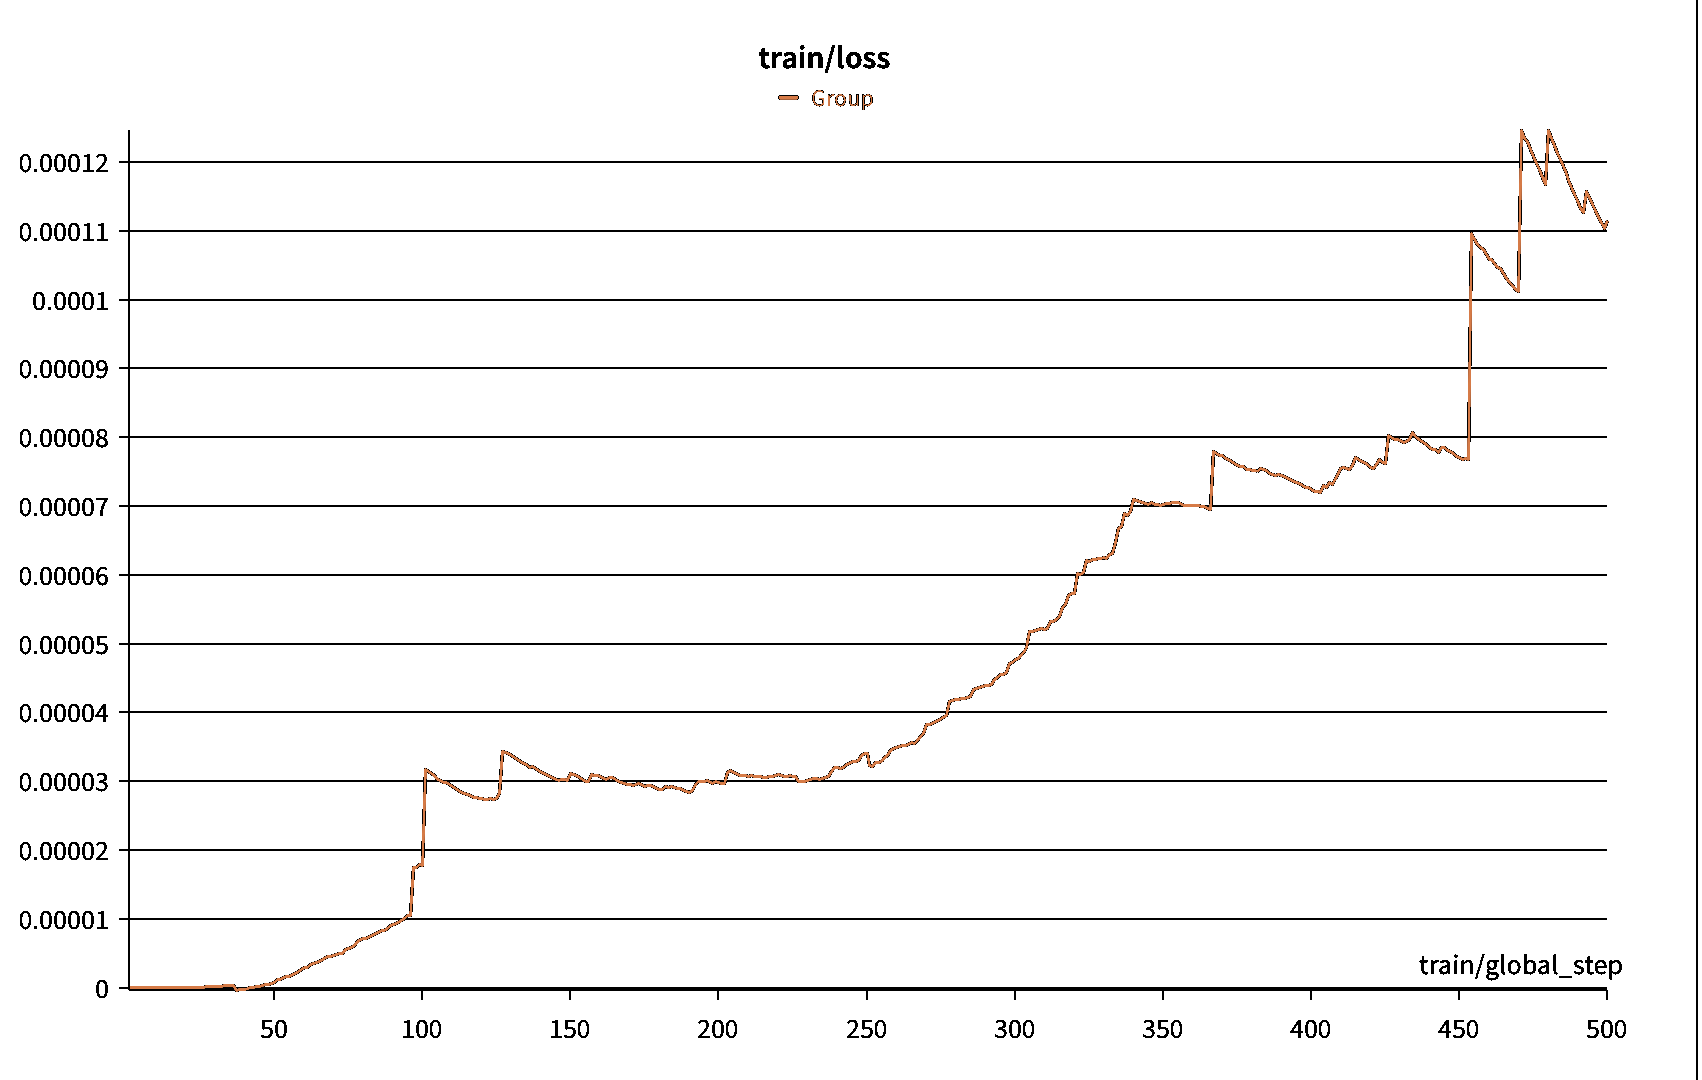
\includegraphics[width=\linewidth]{figures/qwen32b-loss}
    \caption{Loss}
    \label{fig:qwen32b-loss}
  \end{subfigure}
  \hfill
  \begin{subfigure}[b]{0.48\columnwidth}
    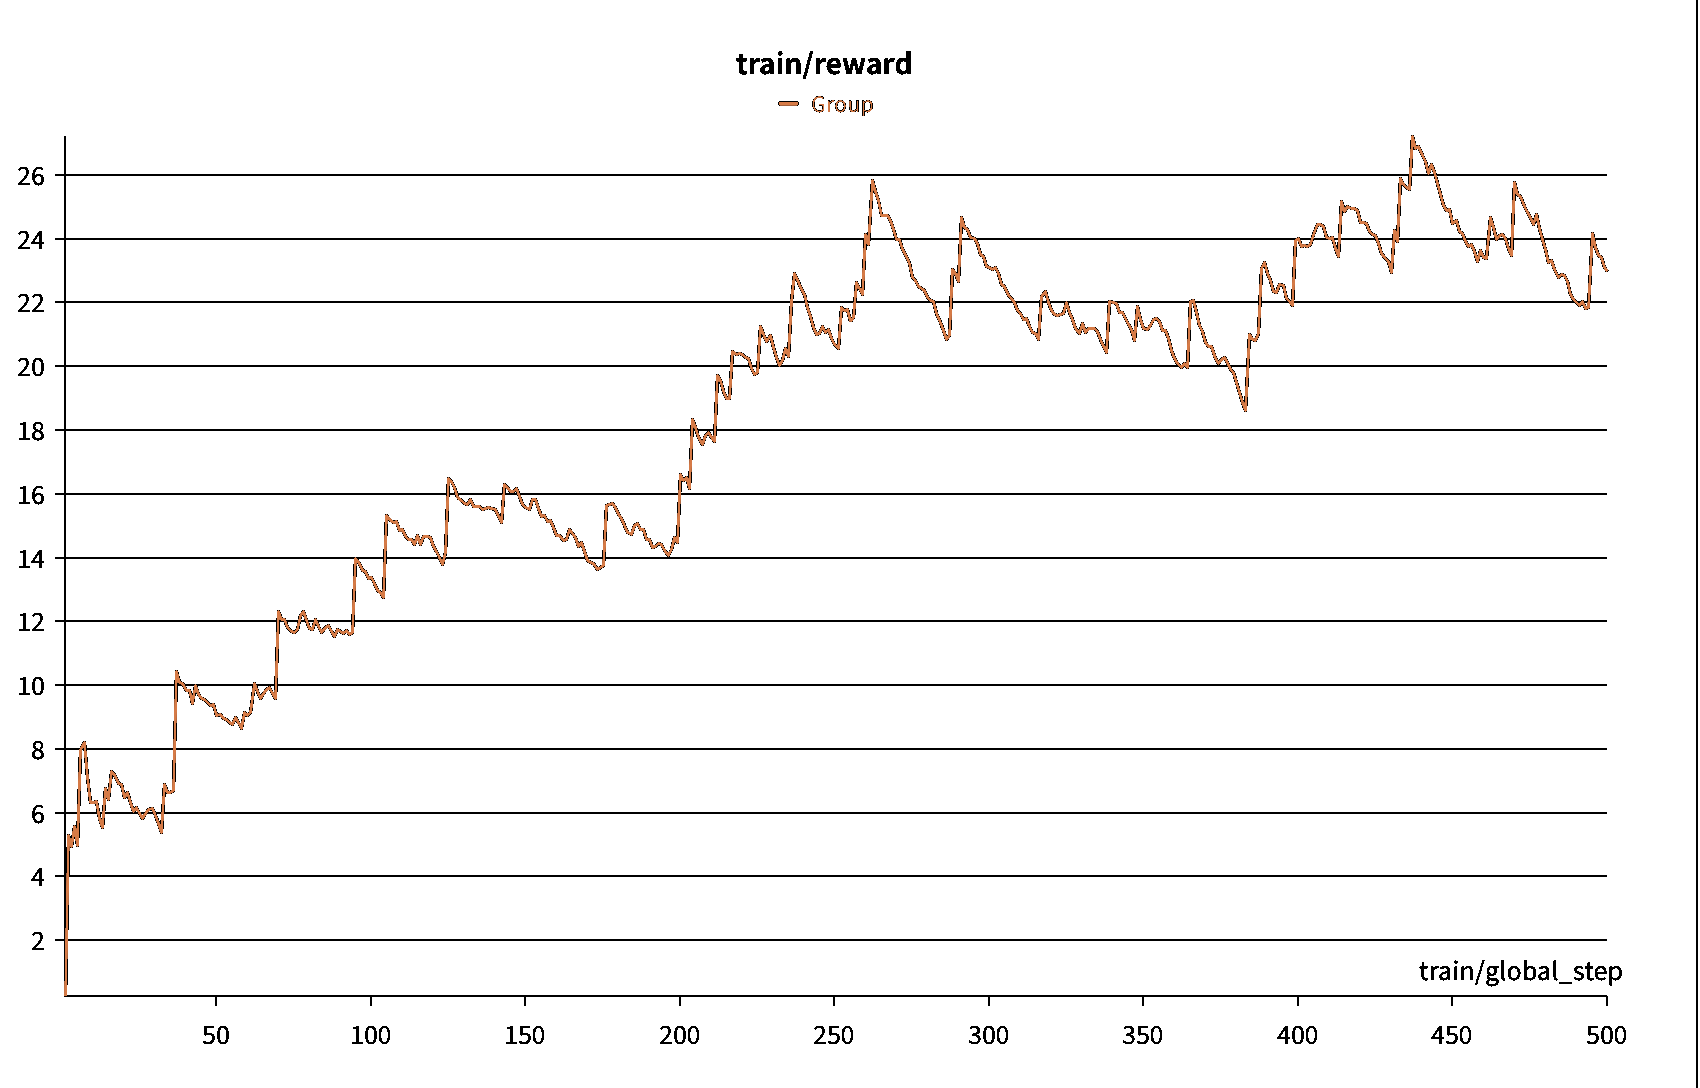
\includegraphics[width=\linewidth]{figures/qwen32b-reward}
    \caption{Mean reward}
    \label{fig:qwen32b-reward}
  \end{subfigure}
  \caption{GRPO fine-tuning curves for Qwen2.5-32B over 500 steps; Qwen2.5-7B and Llama-3.1-8B exhibit the same qualitative behaviour.}
  \label{fig:training-curves}
\end{figure}

\subsubsection{Strategy Generation Performance}
We evaluate each model on 38 stocks with 10 back-testing episodes per stock (380 test
instances per model). Valid strategies are all strategies that executed without error;
Prof.\,\% is profitable strategies as a fraction of all 380 instances;
Mean Ret., Sharpe, and Ann.\ are the mean cumulative return, Sharpe ratio, and annualised
return of a model's valid strategies; and $\Delta$ columns are relative percentage
increases of the fine-tuned model over its base counterpart, computed from the raw
counts. \Cref{tab:model-comparison} shows a significant improvement for all models
across all metrics, except the decrease in mean Sharpe ratio for fine-tuned Llama-3.1-8B,
which remains largely unable to generate profitable strategies, as evidenced by its
negative annualised return and low profitable rate. The fine-tuned Qwen2.5-32B model
achieves the highest profitable rate (62.1\%) and mean return (37.30\%), followed by
fine-tuned Qwen2.5-7B at 58.9\% and 31.55\%; both substantially outperform their base
counterparts.

\begin{table}[t]
  \centering
  \caption{Strategy generation performance of fine-tuned vs.\ base models.}
  \label{tab:model-comparison}
  \resizebox{\columnwidth}{!}{%
  \begin{tabular}{lrrrrrrrrrr}
    \toprule
    Model & Valid & Prof. & Valid.\,(\%) & Mean Ret.\,(\%) & Sharpe & Ann.\,(\%) & Prof.\,\% & $\Delta$\,Valid\,\% & $\Delta$\,Prof.\,\% & $\Delta$\,Ann.\,(\%) \\
    \midrule
    Llama-3.1-8B (base)         &  38 &  12 & 10   & 0.84  & $-$4.62 & $-$2.18 &  3.2 & —        & —        & —        \\
    Llama-3.1-8B (ft.)          & 124 &  68 & 32.6 & 2.17  & $-$5.04 & $-$1.68 & 17.9 & $+$226.3 & $+$466.7 & $+$22.9  \\
    \addlinespace
    Qwen2.5-7B (base)           & 285 & 160 & 75   & 0.62  & $-$5.10 &   1.30  & 42.1 & —        & —        & —        \\
    Qwen2.5-7B (ft.)            & 338 & 224 & 88.9 & 31.55 &   0.08  &   6.98  & 58.9 & $+$18.6  & $+$40.0  & $+$436.9 \\
    \addlinespace
    Qwen2.5-32B (base)          & 357 & 219 & 93.9 & 11.00 & $-$4.06 &   2.35  & 57.6 & —        & —        & —        \\
    Qwen2.5-32B (ft.)           & 371 & 236 & 97.6 & 37.30 &   0.20  &   9.20  & 62.1 & $+$3.9   & $+$7.8   & $+$291.5 \\
    \bottomrule
  \end{tabular}}
\end{table}

\subsubsection{Per-Asset Performance Comparison}
\Cref{tab:per-asset-1,tab:per-asset-comparison} report per-asset trading performance
(ARR\%, SR, MDD\%) for our best fine-tuned models alongside representative baselines drawn
from the FinAgent benchmark~\cite{zhang2024finagent}; ETHUSD is omitted as our evaluation
set did not include cryptocurrency assets, and ``---'' indicates no valid strategy was
produced for that asset. We note that the LLM-based benchmarks consume financial news,
social media, and earnings reports among other sources, while our models use only
quantitative price data, giving those benchmarks a structural information advantage.

\begin{table}[t]
  \centering
  \caption{Per-asset performance (AAPL, AMZN, GOOGL). Baselines from \cite{zhang2024finagent}. \textbf{Bold} = best ARR/SR per asset.}
  \label{tab:per-asset-1}
  \resizebox{\columnwidth}{!}{%
  \begin{tabular}{llrrrrrrrrr}
    \toprule
    & & \multicolumn{3}{c}{AAPL} & \multicolumn{3}{c}{AMZN} & \multicolumn{3}{c}{GOOGL} \\
    \cmidrule(lr){3-5}\cmidrule(lr){6-8}\cmidrule(lr){9-11}
    Cat. & Model & ARR & SR & MDD & ARR & SR & MDD & ARR & SR & MDD \\
    \midrule
    Mkt  & B\&H        & 13.00 & 0.60 & 14.78 & 42.33 & 1.08 & 17.38 & 22.47 & 0.71 & 12.97 \\
    \addlinespace
    ML   & LSTM        & 10.97 & 0.54 & 11.95 & 15.91 & 0.46 & 17.41 & 24.86 & 0.70 & 12.98 \\
    \addlinespace
    RL   & DQN         &  7.92 & 0.40 & 14.88 & 27.43 & 1.17 &  5.27 & 34.40 & 1.39 &  7.15 \\
         & PPO         & 13.26 & 0.61 & 14.78 & 21.17 & 0.70 & 13.84 & 38.29 & 1.30 &  8.45 \\
    \addlinespace
    LLM  & FinGPT      & $-$5.46 & $-$0.17 & 16.23 & 42.93 & 1.10 & 18.94 & 12.28 & 0.44 & 13.00 \\
         & FinMem      & 23.78 & 1.11 & 10.39 & 40.07 & 1.03 & 18.53 & 31.27 & 1.11 &  8.97 \\
         & FinAgent    & \textbf{31.90} & \textbf{1.43} & 10.40 & \textbf{65.10} & 1.61 & 13.20 & \textbf{56.15} & \textbf{1.78} &  8.45 \\
    \midrule
    Ours & Llama (ft.) & {---} & {---} & {---} & 0.24 & $-$1.72 & 0.63 & 0.09 & $-$9.42 & 0.18 \\
         & Q-7B (ft.)  & 25.43 & 1.34 & 15.57 & 19.03 & \textbf{1.62} & 22.16 & 16.11 & 0.94 & 13.02 \\
         & Q-32B (ft.) & 25.23 & 1.34 & 15.57 & 25.10 & 0.49 & 41.41 & 27.41 & 0.96 & 12.87 \\
    \bottomrule
  \end{tabular}}
\end{table}

\begin{table}[t]
  \centering
  \caption{Per-asset performance (MSFT, TSLA). Baselines from \cite{zhang2024finagent}. \textbf{Bold} = best ARR/SR per asset.}
  \label{tab:per-asset-comparison}
  \resizebox{\columnwidth}{!}{%
  \begin{tabular}{llrrrrrr}
    \toprule
    & & \multicolumn{3}{c}{MSFT} & \multicolumn{3}{c}{TSLA} \\
    \cmidrule(lr){3-5}\cmidrule(lr){6-8}
    Cat. & Model & ARR & SR & MDD & ARR & SR & MDD \\
    \midrule
    Mkt  & B\&H        & 22.49 & 0.84 & 12.92 & 37.40 & 0.72 & 32.65 \\
    \addlinespace
    ML   & LSTM        & 18.86 & 0.68 & 11.75 & 17.36 & 0.78 &  4.44 \\
    \addlinespace
    RL   & DQN         & 30.44 & 1.18 & 10.56 & 15.07 & 0.44 & 28.12 \\
         & PPO         & 11.32 & 0.48 & 17.51 & 33.64 & 0.78 & 28.35 \\
    \addlinespace
    LLM  & FinGPT      & 25.10 & 0.97 &  9.84 & 38.43 & 0.75 & 31.47 \\
         & FinMem      & 40.58 & 1.50 &  7.48 & 50.04 & 0.92 & 25.77 \\
         & FinAgent    & \textbf{44.74} & \textbf{1.79} &  5.57 & \textbf{92.27} & \textbf{2.01} & 12.14 \\
    \midrule
    Ours & Llama (ft.) &  4.85 & 0.28 & 13.73 &  1.04 & 0.00 & 17.05 \\
         & Q-7B (ft.)  & 23.26 & 0.70 & 25.60 & 12.85 & 0.92 & 15.72 \\
         & Q-32B (ft.) & 25.99 & 0.79 & 26.65 & 25.41 & 0.35 & 63.55 \\
    \bottomrule
  \end{tabular}}
\end{table}

% ── Section 5 – Conclusion ────────────────────────────────────────────────────
\section{Conclusion}
\label{ch:conclusion}

We explored the application of GRPO to train large language models for financial trading
strategy generation, via a pipeline that prompts the model to generate
Backtrader-compatible strategies, evaluates them by back-testing, and assigns rewards
based on their performance. GRPO fine-tuning significantly improved the
ability of all tested models to generate valid and profitable strategies compared to their
base counterparts, with the fine-tuned Qwen2.5-32B achieving the highest profitable rate
and mean return---suggesting GRPO is an effective method for aligning LLMs with complex,
domain-specific objectives.

Several limitations remain: the reward function does not capture risk-adjusted returns or
drawdown; the back-testing environment omits slippage and transaction costs;
computational cost limited experiments with larger models; and the fine-tuned models often
converge on similar indicator-based strategies---evident in the near-identical AAPL
results of the two Qwen models---leaving the diversity of generated strategies an open
question. Future work could explore
richer reward functions, more realistic market simulation, multi-asset extension, and
alternative algorithms such as Direct Preference Optimisation (DPO) or Group Sequence
Policy Optimisation (GSPO).

% ── Bibliography ─────────────────────────────────────────────────────────────
\bibliographystyle{IEEEtran}
\bibliography{references}

\end{document}
